\section{Benchmarking de Sistemas Similares}\label{cap:benchmarking}

El benchmarking, entendido como la búsqueda de las mejores prácticas que conducen a un desempeño superior (Camp, 1989), se aplicó para comparar el sistema propuesto con cuatro plataformas comerciales de gestión de salones —Fresha, Booksy, AgendaPro y Vagaro— y con la solución actualmente usada por el salón (hoja de cálculo). La selección se basó en su presencia en el mercado hispanohablante o internacional y en que ofrecen funciones de agenda, cobro y comisiones. La información proviene de las páginas oficiales de cada producto, consultadas el 30 de octubre de 2026.


Los criterios de comparación derivan de las necesidades del salón: comisiones configurables, propinas, liquidación de personal, importación desde Excel, funcionamiento sin conexión y modelo de costo. La Tabla~\ref{tab:v4_3} resume los resultados. La expresión «No documentado» indica que la página consultada no menciona la función, lo que no implica necesariamente que el producto carezca de ella.


\vspace{8pt}{\footnotesize\setstretch{1.0}
\begin{longtable}{>{\raggedright\arraybackslash}p{0.1573\dimexpr\linewidth-14\tabcolsep\relax}>{\raggedright\arraybackslash}p{0.1331\dimexpr\linewidth-14\tabcolsep\relax}>{\raggedright\arraybackslash}p{0.1411\dimexpr\linewidth-14\tabcolsep\relax}>{\raggedright\arraybackslash}p{0.1371\dimexpr\linewidth-14\tabcolsep\relax}>{\raggedright\arraybackslash}p{0.1411\dimexpr\linewidth-14\tabcolsep\relax}>{\raggedright\arraybackslash}p{0.1371\dimexpr\linewidth-14\tabcolsep\relax}>{\raggedright\arraybackslash}p{0.1532\dimexpr\linewidth-14\tabcolsep\relax}}
\caption{Comparación de sistemas de gestión para salones de belleza}\label{tab:v4_3}\\
\toprule
\textbf{Criterio} & \textbf{Fresha} & \textbf{Booksy} & \textbf{AgendaPro} & \textbf{Vagaro} & \textbf{Hoja de cálculo (actual)} & \textbf{Lush Beauty (propuesta)} \\
\midrule\endfirsthead
\toprule
\textbf{Criterio} & \textbf{Fresha} & \textbf{Booksy} & \textbf{AgendaPro} & \textbf{Vagaro} & \textbf{Hoja de cálculo (actual)} & \textbf{Lush Beauty (propuesta)} \\
\midrule\endhead
\bottomrule\endfoot
\bottomrule\endlastfoot
Agenda y reservas en línea & Sí & Sí & Sí & Sí & No & Fuera del MVP (futuro) \\
Punto de venta y cierre de caja & Sí & Sí (con procesador de pagos) & Parcial (cierres de caja) & Sí (terminales propias) & Manual & Sí; caja diaria por método de pago \\
Comisiones del personal & No documentado & Sí, automática en cada cobro & Sí, mediante reporte & No documentado & Fórmula fija 35~\% por hoja & Sí; reglas configurables con vigencia \\
Propinas & Parcial (se cobran en la reserva) & Sí, seguimiento automático & No documentado & No documentado & Columna aparte & Sí; ajustables y con política de reparto \\
Liquidación de nómina & No documentado & Parcial (cálculo de comisiones y propinas) & No documentado & No documentado & Manual & Sí; semanal, con deducciones y excedente \\
Importación desde Excel & Parcial (clientes e inventario) & No documentado & No documentado & No documentado & No aplica & Sí; vista previa y detección de duplicados \\
Uso sin conexión & No documentado & No documentado & No documentado & No documentado & Sí (archivo local) & Sí; cola local y sincronización \\
Auditoría de cambios & No documentado & No documentado & No documentado & No documentado & No & Sí; bitácora inmutable \\
Modelo de costo & Suscripción mensual con complementos & USD 29,99 al mes más USD 20 por usuario adicional & Planes por suscripción (precios no visibles) & Suscripción mensual (USD 23,99) más comisión de procesamiento & Sin costo adicional & Desarrollo propio; costo de alojamiento \\
\end{longtable}}
\nota{Elaboración propia a partir de las páginas oficiales de Fresha (s. f.), Booksy (s. f.), AgendaPro (s. f.) y Vagaro (s. f.), consultadas el 30 de octubre de 2026. Los precios son referenciales y están sujetos a cambios.}

De la comparación se desprenden tres conclusiones. Primero, las plataformas comerciales priorizan la agenda y el cobro con tarjeta, y tratan la liquidación de personal de forma parcial: la mayoría documenta el cálculo de comisiones, pero no un proceso de liquidación periódica con deducciones. Segundo, ninguna de las páginas consultadas describe la importación de planillas heredadas de un salón ni el registro sin conexión, dos requisitos críticos para una microempresa que opera desde el teléfono y que migra desde Excel. Tercero, el modelo de costo en dólares y por usuario adicional puede resultar oneroso para un salón de tres personas, además de que las reglas de comisión propias del negocio (porcentaje sobre precio de lista, excedente de deducción) no son parametrizables en el grado requerido.


Estas brechas justifican el desarrollo de una solución propia, enfocada en caja y nómina, que incorpore lo que las plataformas comerciales ya resolvieron bien —cobro, comisiones automáticas, aplicación móvil— y cubra lo no documentado en ellas. La agenda de reservas se incorporará en una etapa posterior, aprovechando que el catálogo se expondrá mediante una interfaz de consulta pública.


La Figura~\ref{fig:v4_2} muestra la arquitectura propuesta: una aplicación cliente instalable, una interfaz de programación (API) con módulos de dominio y una base de datos relacional con aislamiento por inquilino y bitácora inmutable.


\begin{figure}[H]
\caption{Arquitectura propuesta del sistema Lush Beauty}\label{fig:v4_2}
\centering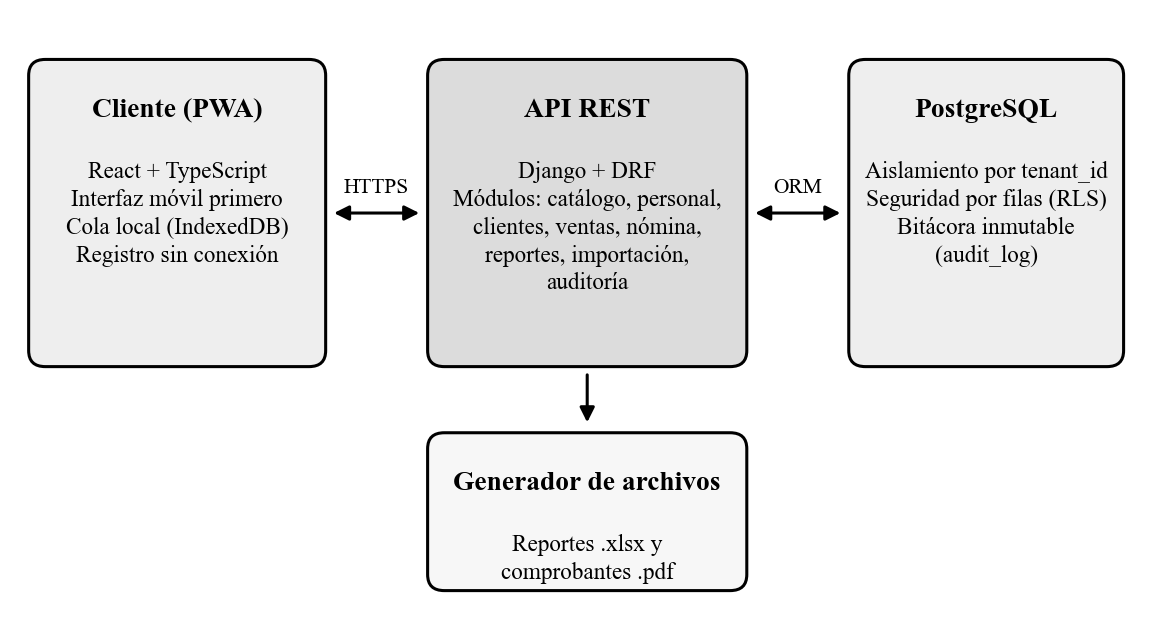
\includegraphics[width=0.9\linewidth]{img/fig_arquitectura_v4.png}
\end{figure}
\nota{Elaboración propia. PWA: aplicación web progresiva; RLS: seguridad a nivel de fila.}

\subsection{Comparación por problema y enfoque}

Para precisar la diferenciación, la Tabla~\ref{tab:dss_3} contrasta cada necesidad del salón con el enfoque de Lush Beauty Smart. La ausencia de una función en la documentación consultada de las plataformas comerciales no demuestra que el proveedor carezca de ella; el contraste se limita a cómo la propuesta prioriza necesidades específicas del negocio.

\vspace{8pt}{\small\setstretch{1.0}
\begin{longtable}{>{\raggedright\arraybackslash}p{0.3333\dimexpr\linewidth-6\tabcolsep\relax}>{\raggedright\arraybackslash}p{0.3333\dimexpr\linewidth-6\tabcolsep\relax}>{\raggedright\arraybackslash}p{0.3333\dimexpr\linewidth-6\tabcolsep\relax}}
\caption{Comparación por problema y enfoque}\label{tab:dss_3}\\
\toprule
\textbf{Criterio} & \textbf{Necesidad de Lush Beauty} & \textbf{Enfoque de la propuesta} \\
\midrule\endfirsthead
\toprule
\textbf{Criterio} & \textbf{Necesidad de Lush Beauty} & \textbf{Enfoque de la propuesta} \\
\midrule\endhead
\bottomrule\endfoot
\bottomrule\endlastfoot
Liquidación semanal & Comisión, propinas y deducciones & Motor versionado y detalle por línea \\
Conciliación & Efectivo, QR y transferencias & Cierre diario con conciliación \\
Migración de Excel & Nombres inconsistentes y columnas dispares & Previsualización y validación asistida \\
Uso móvil sin conexión & Registro durante la atención & PWA con cola idempotente \\
Asistencia financiera & Interpretar causas de variaciones & Lush Insight con consultas permitidas \\
Automatización & Entrega de reportes y alertas & Flujos n8n con eventos aprobados \\
\end{longtable}}
\nota{Elaboración propia. No implica ausencia de estas capacidades en productos comerciales.}

\subsection{Propuesta de valor}

Lush Beauty Smart se posiciona como una plataforma especializada en el flujo financiero de pequeñas empresas de belleza. Su diferenciación propuesta se resume en registrar con rapidez, calcular con exactitud, explicar con evidencia y automatizar sin perder control. La posibilidad de operar múltiples salones mediante aislamiento de datos constituye una opción de expansión futura y no una característica que sea necesario comercializar o probar a escala durante la feria.


\subsection{Diferenciación como sistema de soporte para decisiones}

La comparación comercial realizada en el benchmarking se centra en agenda, caja, comisiones, propinas y reportes. La ampliación DSS no afirma que los productos comparados carezcan de funciones avanzadas: propone una diferenciación evaluable para el caso de estudio, consistente en simular alternativas económicas con reglas visibles y evaluar después los resultados de las decisiones. El benchmarking de estas nuevas capacidades requerirá una verificación específica si se utiliza para afirmar superioridad de mercado.

